\subsection{Koordinatsystem}
\label{Koordinatsystem}

Det koordinatsystem som brukar användas i Matematik 2B är tvådimensionellt och består av två reella tallinjer som är vinkelräta och möter varann i \textit{origo} där båda är $0$.

En position, eller \textit{koordinat}, i koordinatsystemet anges som $(x, y)$ där $x$ anger positionen längs den horisontella \textit{x-axeln} och $y$ anger positionen längs den vertikala \textit{y-axeln}.

Här är ett exempel på en koordinat $A = (3, 1)$ i detta koordinatsystem:

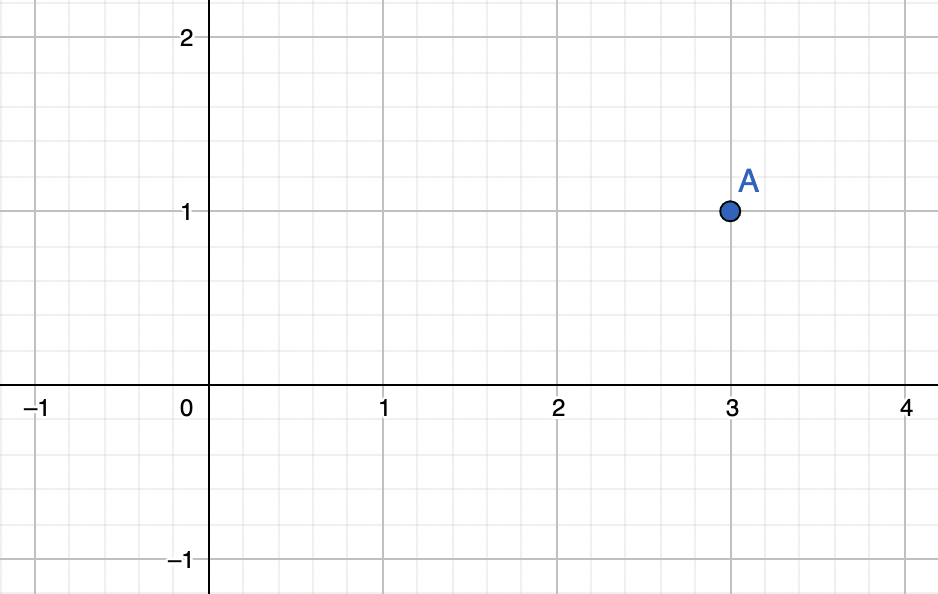
\includegraphics[width=\textwidth]{img/1.png}

\subsubsection{Avståndsformeln}

Avståndet mellan två punkter i koordinatsystemet från \ref{Koordinatsystem} kan beräknas med hjälp av Pythagoras Sats från \ref{Pythagoras Sats}. Om vi börjar med två koordinater, $A=(2,2)$ och $B=(4,3)$

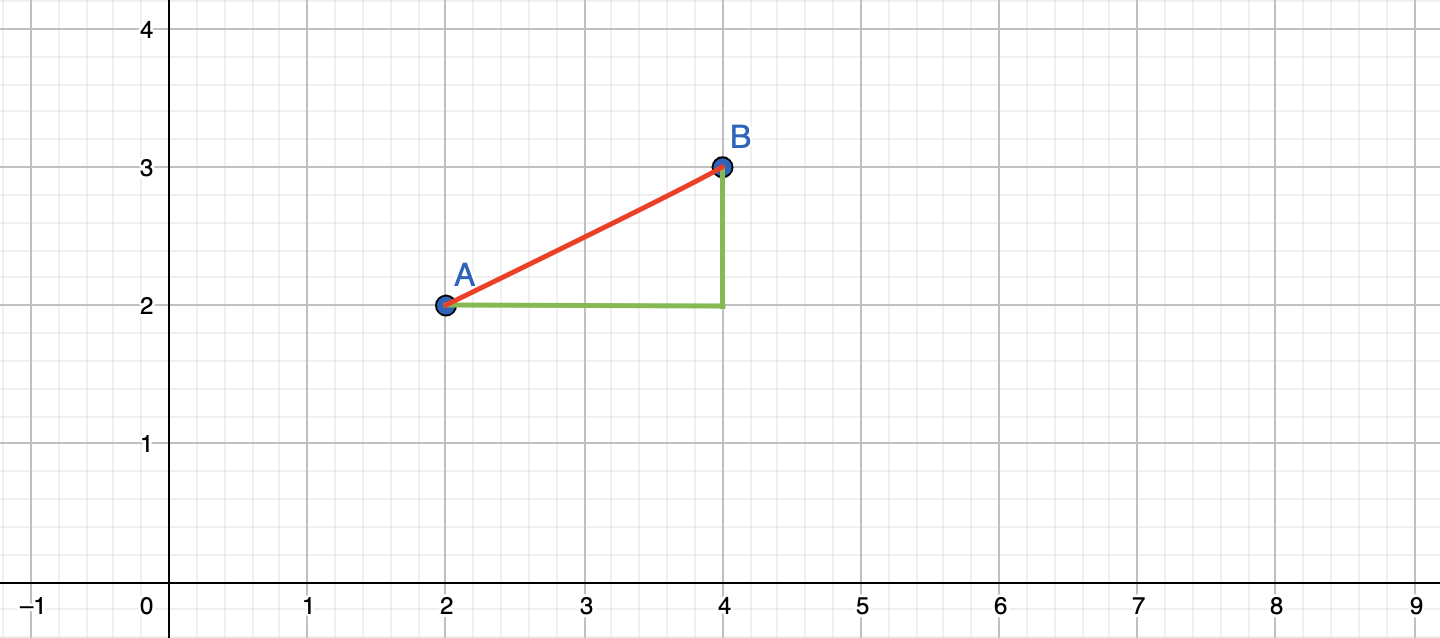
\includegraphics[width=\textwidth]{img/3.png}

Så kan vi se att de bildar en rätvinklig triangel, där en av kateterna är längs x-axeln och den andra längs y-axeln. Avståndet är då den röda linjen. Om vi vet längden av de två kateterna, så kan vi veta längden för hypotenusan, med pythagoras sats.

Längden av kateten längs x-axeln, som vi kan kalla $a$, är då absolutvärdet\footnote{absolutvärdet är distansen från $0$ på tallinjen, så t.ex är |-5| = 5. I fallet ovan så använder vi absolutvärdet då en distans aldrig kan vara negativ, men en differens mellan delar av två koordinater kan det.} av differensen mellan koordinaternas x-värden, så den kateten är

\begin{align}
	a = \\
	|2-4| = \\
	|-2| = \\
	2 \text{ (l.e)}
\end{align}

Vi kan göra exakt samma sak för kateten längs y-axeln, som vi kan kalla för $b$.

\begin{align}
	b = \\
	|2-3| = \\
	|-1| = \\
	1 \text{ (l.e)}
\end{align}

Då vi vill veta längden av hypotenusan, vilket är avståndet mellan koordinaterna, så kan vi lösa ut variabeln $c$ ur pythagoras sats, och sedan sätta in de värden vi har tagit fram.

\begin{align}
	a^2+b^2=c^2 \\
	c = \sqrt{a^2+b^2} \\
	c = \sqrt{2^2+1^2} \\
	c = \sqrt{5} \text{ (l.e)}
\end{align}

\subsubsection{Formeln}

Vi kan nu generalisera det vi gjorde ovan. 

Låt $A=(a,b)$, $B=(c,d)$ och $l$ avståndet mellan koordinaterna. Då är

\begin{align}
	l = \sqrt{|a-c|^2+|b-d|^2}
\end{align}

och då absolutvärdefunktionen inte behövs, då vi ändå kvadrerar båda termerna, så kan vi förenkla detta till

\begin{align}
	l = \sqrt{(a-c)^2+(b-d)^2}.
\end{align}

\subsection{Funktion}

En funktion inom Matematik 2B är något som översätter ett nummer till ett annat. Ett exempel är denna funktion $f$,

\begin{align}
	f(x) = \frac{1}{2}x-1
\end{align}

som översätter $2$ till $0$, eller $4$ till $1$.

vi kan rita up $f$ grafiskt i koordinatsystemet från \ref{Koordinatsystem}, genom att låta $f(x) = y$.

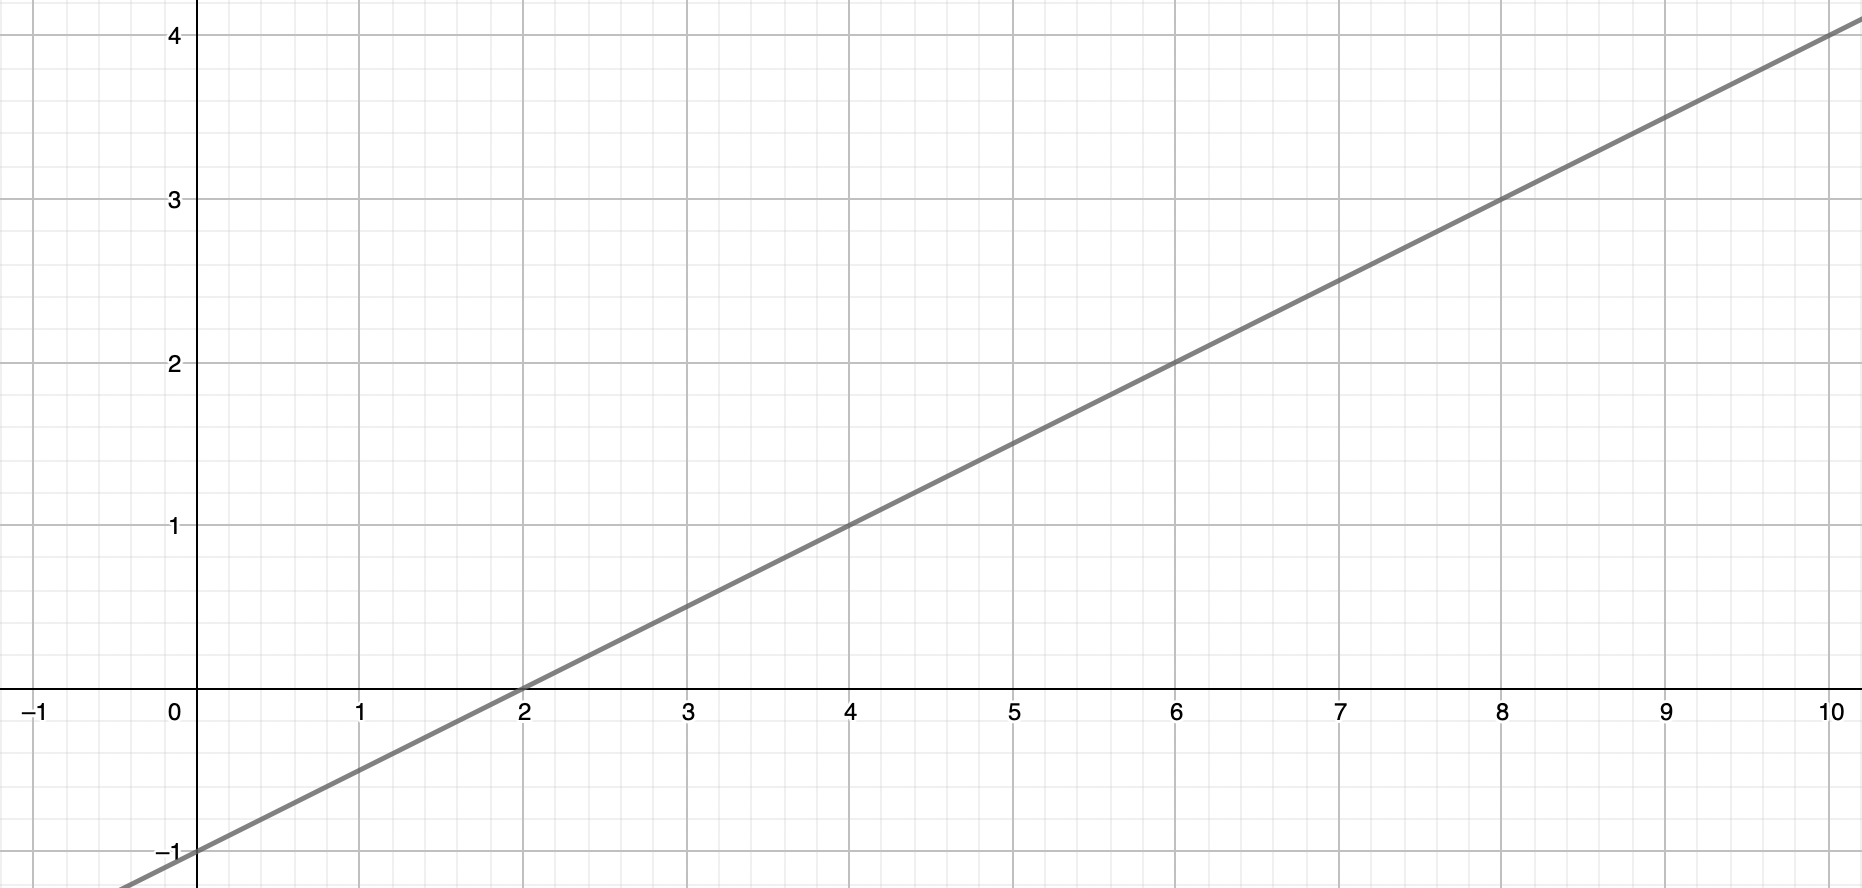
\includegraphics[width=\textwidth]{img/2.png}


























